% Also note that the "draftcls" or "draftclsnofoot", not "draft", option
% should be used if it is desired that the figures are to be displayed in
% draft mode.

\documentclass[conference]{IEEEtran}
% Add the compsoc option for Computer Society conferences.
%
% If IEEEtran.cls has not been installed into the LaTeX system files,
% manually specify the path to it like:
% \documentclass[conference]{../sty/IEEEtran}

	% Some very useful LaTeX packages include:
	% (uncomment the ones you want to load)

	% *** MISC UTILITY PACKAGES ***
	%\usepackage{ifpdf}
		% Heiko Oberdiek's ifpdf.sty is very useful if you need conditional compilation based on whether 
		% the output is pdf or dvi.
		% usage:
		% \ifpdf
		%   % pdf code
		% \else
		%   % dvi code
		% \fi
		% The latest version of ifpdf.sty can be obtained from: http://www.ctan.org/tex-archive/macros/latex/contrib/oberdiek/
		% Also, note that IEEEtran.cls V1.7 and later provides a builtin \ifCLASSINFOpdf conditional that 
		% works the same way. When switching from latex to pdflatex and vice-versa, the compiler may
		% have to be run twice to clear warning/error messages.

	% *** CITATION PACKAGES ***
	\usepackage{cite}
		% cite.sty was written by Donald Arseneau
		% V1.6 and later of IEEEtran pre-defines the format of the cite.sty package
		% \cite{} output to follow that of IEEE. Loading the cite package will
		% result in citation numbers being automatically sorted and properly
		% "compressed/ranged". e.g., [1], [9], [2], [7], [5], [6] without using
		% cite.sty will become [1], [2], [5]--[7], [9] using cite.sty. cite.sty's
		% \cite will automatically add leading space, if needed. Use cite.sty's
		% noadjust option (cite.sty V3.8 and later) if you want to turn this off.
		% cite.sty is already installed on most LaTeX systems. Be sure and use
		% version 4.0 (2003-05-27) and later if using hyperref.sty. cite.sty does
		% not currently provide for hyperlinked citations.
		% The latest version can be obtained at:
		% http://www.ctan.org/tex-archive/macros/latex/contrib/cite/
		% The documentation is contained in the cite.sty file itself.

	% *** GRAPHICS RELATED PACKAGES ***
	\ifCLASSINFOpdf
		\usepackage[pdftex]{graphicx}
			% declare the path(s) where your graphic files are
			% \graphicspath{{../pdf/}{../jpeg/}}
			% and their extensions so you won't have to specify these with
			% every instance of \includegraphics
			% \DeclareGraphicsExtensions{.pdf,.jpeg,.png}
	\else
		% or other class option (dvipsone, dvipdf, if not using dvips). graphicx
		% will default to the driver specified in the system graphics.cfg if no
		% driver is specified.
		% \usepackage[dvips]{graphicx}
		% declare the path(s) where your graphic files are
		% \graphicspath{{../eps/}}
		% and their extensions so you won't have to specify these with
		% every instance of \includegraphics
		% \DeclareGraphicsExtensions{.eps}
	\fi
		% graphicx was written by David Carlisle and Sebastian Rahtz. It is
		% required if you want graphics, photos, etc. graphicx.sty is already
		% installed on most LaTeX systems. The latest version and documentation can
		% be obtained at: 
		% http://www.ctan.org/tex-archive/macros/latex/required/graphics/
		% Another good source of documentation is "Using Imported Graphics in
		% LaTeX2e" by Keith Reckdahl which can be found as epslatex.ps or
		% epslatex.pdf at: http://www.ctan.org/tex-archive/info/
		% latex, and pdflatex in dvi mode, support graphics in encapsulated
		% postscript (.eps) format. pdflatex in pdf mode supports graphics
		% in .pdf, .jpeg, .png and .mps (metapost) formats. Users should ensure
		% that all non-photo figures use a vector format (.eps, .pdf, .mps) and
		% not a bitmapped formats (.jpeg, .png). IEEE frowns on bitmapped formats
		% which can result in "jaggedy"/blurry rendering of lines and letters as
		% well as large increases in file sizes.
		% You can find documentation about the pdfTeX application at:
		% http://www.tug.org/applications/pdftex

	% *** MATH PACKAGES ***
	\usepackage[cmex10]{amsmath}
		% A popular package from the American Mathematical Society that provides
		% many useful and powerful commands for dealing with mathematics. If using
		% it, be sure to load this package with the cmex10 option to ensure that
		% only type 1 fonts will utilized at all point sizes. Without this option,
		% it is possible that some math symbols, particularly those within
		% footnotes, will be rendered in bitmap form which will result in a
		% document that can not be IEEE Xplore compliant!
		%
		% Also, note that the amsmath package sets \interdisplaylinepenalty to 10000
		% thus preventing page breaks from occurring within multiline equations. Use:
		%\interdisplaylinepenalty=2500
		% after loading amsmath to restore such page breaks as IEEEtran.cls normally
		% does. amsmath.sty is already installed on most LaTeX systems. The latest
		% version and documentation can be obtained at:
		% http://www.ctan.org/tex-archive/macros/latex/required/amslatex/math/
	\usepackage{amssymb}

	% *** SPECIALIZED LIST PACKAGES ***
	\usepackage{algorithmic}
		% algorithmic.sty was written by Peter Williams and Rogerio Brito.
		% This package provides an algorithmic environment fo describing algorithms.
		% You can use the algorithmic environment in-text or within a figure
		% environment to provide for a floating algorithm. Do NOT use the algorithm
		% floating environment provided by algorithm.sty (by the same authors) or
		% algorithm2e.sty (by Christophe Fiorio) as IEEE does not use dedicated
		% algorithm float types and packages that provide these will not provide
		% correct IEEE style captions. The latest version and documentation of
		% algorithmic.sty can be obtained at:
		% http://www.ctan.org/tex-archive/macros/latex/contrib/algorithms/
		% There is also a support site at:
		% http://algorithms.berlios.de/index.html
		% Also of interest may be the (relatively newer and more customizable)
		% algorithmicx.sty package by Szasz Janos:
		% http://www.ctan.org/tex-archive/macros/latex/contrib/algorithmicx/

	% *** ALIGNMENT PACKAGES ***
	\usepackage{array}
		% Frank Mittelbach's and David Carlisle's array.sty patches and improves
		% the standard LaTeX2e array and tabular environments to provide better
		% appearance and additional user controls. As the default LaTeX2e table
		% generation code is lacking to the point of almost being broken with
		% respect to the quality of the end results, all users are strongly
		% advised to use an enhanced (at the very least that provided by array.sty)
		% set of table tools. array.sty is already installed on most systems. The
		% latest version and documentation can be obtained at:
		% http://www.ctan.org/tex-archive/macros/latex/required/tools/
	\usepackage{mdwmath}
	\usepackage{mdwtab}
		% Also highly recommended is Mark Wooding's extremely powerful MDW tools,
		% especially mdwmath.sty and mdwtab.sty which are used to format equations
		% and tables, respectively. The MDWtools set is already installed on most
		% LaTeX systems. The lastest version and documentation is available at:
		% http://www.ctan.org/tex-archive/macros/latex/contrib/mdwtools/
		% IEEEtran contains the IEEEeqnarray family of commands that can be used to
		% generate multiline equations as well as matrices, tables, etc., of high
		% quality.
	\usepackage{eqparbox}
		% Also of notable interest is Scott Pakin's eqparbox package for creating
		% (automatically sized) equal width boxes - aka "natural width parboxes".
		% Available at:
		% http://www.ctan.org/tex-archive/macros/latex/contrib/eqparbox/

	% *** SUBFIGURE PACKAGES ***
	%\usepackage[tight,footnotesize]{subfigure}
		% subfigure.sty was written by Steven Douglas Cochran. This package makes it
		% easy to put subfigures in your figures. e.g., "Figure 1a and 1b". For IEEE
		% work, it is a good idea to load it with the tight package option to reduce
		% the amount of white space around the subfigures. subfigure.sty is already
		% installed on most LaTeX systems. The latest version and documentation can
		% be obtained at:
		% http://www.ctan.org/tex-archive/obsolete/macros/latex/contrib/subfigure/
		% subfigure.sty has been superceeded by subfig.sty.
	%\usepackage[caption=false]{caption}
	%\usepackage[font=footnotesize]{subfig}
		% subfig.sty, also written by Steven Douglas Cochran, is the modern
		% replacement for subfigure.sty. However, subfig.sty requires and
		% automatically loads Axel Sommerfeldt's caption.sty which will override
		% IEEEtran.cls handling of captions and this will result in nonIEEE style
		% figure/table captions. To prevent this problem, be sure and preload
		% caption.sty with its "caption=false" package option. This is will preserve
		% IEEEtran.cls handing of captions. Version 1.3 (2005/06/28) and later 
		% (recommended due to many improvements over 1.2) of subfig.sty supports
		% the caption=false option directly:
	%\usepackage[caption=false,font=footnotesize]{subfig}
		% The latest version and documentation can be obtained at:
		% http://www.ctan.org/tex-archive/macros/latex/contrib/subfig/
		% The latest version and documentation of caption.sty can be obtained at:
		% http://www.ctan.org/tex-archive/macros/latex/contrib/caption/

	% *** FLOAT PACKAGES ***
	%\usepackage{fixltx2e}
		% fixltx2e, the successor to the earlier fix2col.sty, was written by
		% Frank Mittelbach and David Carlisle. This package corrects a few problems
		% in the LaTeX2e kernel, the most notable of which is that in current
		% LaTeX2e releases, the ordering of single and double column floats is not
		% guaranteed to be preserved. Thus, an unpatched LaTeX2e can allow a
		% single column figure to be placed prior to an earlier double column
		% figure. The latest version and documentation can be found at:
		% http://www.ctan.org/tex-archive/macros/latex/base/
	%\usepackage{stfloats}
		% stfloats.sty was written by Sigitas Tolusis. This package gives LaTeX2e
		% the ability to do double column floats at the bottom of the page as well
		% as the top. (e.g., "\begin{figure*}[!b]" is not normally possible in
		% LaTeX2e). It also provides a command:
		%\fnbelowfloat
		% to enable the placement of footnotes below bottom floats (the standard
		% LaTeX2e kernel puts them above bottom floats). This is an invasive package
		% which rewrites many portions of the LaTeX2e float routines. It may not work
		% with other packages that modify the LaTeX2e float routines. The latest
		% version and documentation can be obtained at:
		% http://www.ctan.org/tex-archive/macros/latex/contrib/sttools/
		% Documentation is contained in the stfloats.sty comments as well as in the
		% presfull.pdf file. Do not use the stfloats baselinefloat ability as IEEE
		% does not allow \baselineskip to stretch. Authors submitting work to the
		% IEEE should note that IEEE rarely uses double column equations and
		% that authors should try to avoid such use. Do not be tempted to use the
		% cuted.sty or midfloat.sty packages (also by Sigitas Tolusis) as IEEE does
		% not format its papers in such ways.

	% *** PDF, URL AND HYPERLINK PACKAGES ***
	%\usepackage{url}
		% url.sty was written by Donald Arseneau. It provides better support for
		% handling and breaking URLs. url.sty is already installed on most LaTeX
		% systems. The latest version can be obtained at:
		% http://www.ctan.org/tex-archive/macros/latex/contrib/misc/
		% Read the url.sty source comments for usage information. Basically,
		% \url{my_url_here}.
		% *** Do not adjust lengths that control margins, column widths, etc. ***
		% *** Do not use packages that alter fonts (such as pslatex).         ***
		% There should be no need to do such things with IEEEtran.cls V1.6 and later.
		% (Unless specifically asked to do so by the journal or conference you plan
		% to submit to, of course. )

	% *** LANGUAGE PACKAGES ***
		\usepackage[latin1]{inputenc}
		\usepackage[english]{babel}

%	CORRECTION FOR HYPERNATION	
	\hyphenation{op-tical net-works semi-conduc-tor tran-si-cio-nes}

%	DOCUMENT BEGINING
	\begin{document}		
	
	%	TITLE AND AUTHORS
		%	TITLE
	% paper title
	% can use linebreaks \\ within to get better formatting as desired
		\title{Execution of Timed Petri Nets with IP cores}

%	AUTHORS
	% author names and affiliations
	% use a multiple column layout for up to three different affiliations

	% conference papers do not typically use \thanks and this command
	% is locked out in conference mode. If really needed, such as for
	% the acknowledgment of grants, issue a \IEEEoverridecommandlockouts
	% after \documentclass

	% for over three affiliations, or if they all won't fit within the width
	% of the page, use this alternative format:
	% 
	\author{
		\IEEEauthorblockN{Orlando Micolini}
		\IEEEauthorblockA{
			Laboratorio de Arquitectura \\ de Computadoras\\
			FCEFyN-UNC\\
			C�rdoba, Argentina\\
			Email: omicolini@compuar.com
		}	
	\and
		\IEEEauthorblockN{Julian Nonino}
		\IEEEauthorblockA{
			Laboratorio de Arquitectura \\ de Computadoras\\
			FCEFyN-UNC\\
			C�rdoba, Argentina\\
			Email: noninojulian@gmail.com
		}	
		\and
		\IEEEauthorblockN{Carlos Renzo Pisetta}
		\IEEEauthorblockA{
			Laboratorio de Arquitectura \\ de Computadoras\\
			FCEFyN-UNC\\
			C�rdoba, Argentina\\
			Email: renzopisetta@gmail.com
		}	
	}

	% use for special paper notices
	%\IEEEspecialpapernotice{(Invited Paper)}

	% make the title area
		\maketitle
		
	% For peer review papers, you can put extra information on the cover
	% page as needed:
	% \ifCLASSOPTIONpeerreview
	% \begin{center} \bfseries EDICS Category: 3-BBND \end{center}
	% \fi
	%
	% For peerreview papers, this IEEEtran command inserts a page break and
	% creates the second title. It will be ignored for other modes.
		\IEEEpeerreviewmaketitle
		
	%	ABSTRACT
		\begin{abstract}
	%\boldmath.
	
	In this article, we present a Timed Petri Nets processor wich can be can be directly programmed 
	using vectors and matrices of Petri Nets formalism. This processor can leverage the power of Petri
	Nets for modeling real-time systems and formally verify their properties, which prevent programming
	errors.
	\\
	
	The Petri Nets processor was developed as an IP-core to be inserted in a multi-core system.
	Therefore, we can model the system requirements with Petri Nets, formally verifying all its
	properties and using the IP-core to implement the system is possible to ensure that all properties
	will be met.
	
\end{abstract}
% IEEEtran.cls defaults to using nonbold math in the Abstract.
% This preserves the distinction between vectors and scalars. However,
% if the conference you are submitting to favors bold math in the abstract,
% then you can use LaTeX's standard command \boldmath at the very start
% of the abstract to achieve this. Many IEEE journals/conferences frown on
% math in the abstract anyway.

\begin{IEEEkeywords}
	Multi-Core, Petri Net, Processor.
\end{IEEEkeywords}

	%	INTRODUCTION
		%TODO translate this file
		\section{Introduction}
	\IEEEPARstart{T}{he} computer systems are complex as much its structure as its behavior, even 
	more when they have a great number of states and many combinations of data and input events.

Develop solutions of complex and critical systems for give a solution a real-time systems have 
 problems such as: the inherent complexity of the specification, the coordination of concurrent 
 tasks, the lack of portable algorithms, standardized environments, software and development tools.

And taking into account unambiguous trends in the hardware design, which indicate that one processor
 may not be able to keep pace with increase performance. Therefore the evolution of the processors 
 is consequence of the greater integration and composition of different types of functionalities 
 integrated into a single processor. Even more today, the availability of transistors has made 
 possible to integrate several processor cores on a single chip, which has resulted in the 
 development of Multi-Core technology \cite{hennessypatterson}.
 
Diminishing returns of Instruction Level Parallelism (ILP) and the cost of the increase of frequency,
 mainly due to power limitations (suggests that a 1\% increase in clock speed results in a power 
 increase of 3\%) \cite{domeika}, leads to the use of multicore processors to improve performance. 
 This increase deficiency results in lower run times, lower consumption, lower energy density, lower
 latency and higher bandwidth inter-core communications.
    
Therefore multi-core processors are a proposal to obtain higher performance. This mainly involves 
 lower execution time, energy consumption, energy density, latency and more bandwidth inter-core 
 communications. Furthermore, the heterogeneous multi-core systems have the advantage of employing 
 specialized cores, each of them designed for specific tasks. That is, optimized for a particular 
 need. These processors have the ability to use the available hardware resources when they are 
 specifically required by the software \cite{sriram}.

In order to increase performance, these systems make use of multi-threading and/or multi-tasking 
 allowing take advantage of the multi-cores. However, it takes more effort to design applications 
 because they must provide solution to the problems of concurrent systems.

That is the reason why with these processors, the parallel programming is essential for improving 
 the performance in all segments of software development and even more so in the segment of real-time
 systems.
 
At the Computer Architectures Laboratory of the FCEFyN-UNC a Petri processor has been developed to 
 directly execute ordinary Petri Nets. In this article, we present a new Petri Nets Processor capable
 to execute Time Petri Nets and to be programmed directly with the vectors and matrixes that define 
 the system and its state.
	


		
		\section{Objetives}

	\subsection{Main Objective} 
	The main objective of this work is to design and implement a Petri Nets Processor capable to 
	execute the Time Petri Nets semantics and to be programmed directly from the model's state 
	equations.
	
	\subsection{Secondary Objectives}
	The secondary objectives are:
	\begin{itemize}
        \item Briefly describe Time Petri Nets in order to implement a processor capable of execute them.
        \item Keep executing ordinary Petri Nets with time parameters on two processor clock cycles.
        \item Implement the Time Petri Nets Processor as an IP-core.
	\end{itemize}
	

	%	PETRI NETS CONSIDERING TIME
		\section{Petri Nets Considering Time}
	
	In the Ordinary Petri Nets formalism, the time is not consider and this results in indeterminism 
	regarding the time. It is not specified when a sensibilized transition will be fired or even if it
	will be fired. Neither can be said which transition from a group of transitions in conflict will 
	be fired \cite{garciaizquierdo}.
	
	There are three different interpretations about how the time should be consider. All of them have 
	focus on reduce the indeterminism regarding time in Petri Nets.
	\begin{enumerate}
	  	\renewcommand{\theenumi}{\Alph{enumi}}
	  	\item \underline{Stochastic Petri Net}
	  		\\
			Introduces a stochastic estimation on the instant of firing of a transition.
		\item \underline{Timed Petri Net}
			\\
			Introduces a time condition which specifies the duration of the transition.
		\item \underline{Time Petri Net}
			\\
			Introduce temporary dimensions between which the transition should be fired.
	\end{enumerate}
		
	\begin{figure}[h]
		\centering
		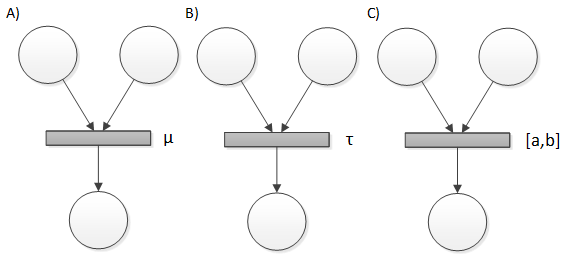
\includegraphics[width=1\linewidth]{./img/Petri16}
		\caption{Different ways to intruduce time in Petri Nets}
		\label{fig:Petri16}
	\end{figure}
	
	The temporal parameters associated with transitions can be interpreted in these three different
	ways\footnotemark:
	
	\footnotetext{ $\bullet t$ is the set of places that are inputs to a
	transition, mathematically defined as: $\bullet t = \{ p \in P : (p , t) \in F \}$.
	
	$t \bullet$ is the set of positions that are outputs of a transition, mathematically defined as: 
		$t \bullet = \{ p \in P : (t , p) \in F \}$.
	
	$F$ is the set of arcs, input and output to the transitions-
	}	
	
	\begin{enumerate}
	  	\item Generalised Stochastic Petri Nets (GSPNs) \cite{gspn} have two different types of 
	  		transitions: immediate transitions and timed transitions. When a transition \emph{t} is
	  		sensitized, its firing could be:
			\begin{enumerate}
			  	\item with a duration equal to zero if the transition \emph{t} is immediate.
			  	\item after lapse of a random time. This random time is expressed by an exponential 
			  	distribution. The A net from the figure \ref{fig:Petri16} graphically represents an stochastic
			  	timed transition where its probability to be fired is represented by $\mu$.
			\end{enumerate}
		\item Timed Petri Nets have two different types of transitions: immediate transitions and timed
			transitions. When a transition \emph{t} is sensitized, its firing could be:
			\begin{enumerate}
			  	\item with a duration equal to zero if the transition \emph{t} is immediate.
			  	\item with immediate removal of tokens from $\bullet t$ set but placing the tokens in 
			  	the $t \bullet$ that only after time $\tau$ has elapsed. Meanwhile, the transition 
			  	can not be sensitized. The B net from the figure \ref{fig:Petri16} graphically represents 
			  	a timed transition with a delay equal to $\tau$.
			\end{enumerate}
		\item Timed Petri Nets have two different types of transitions: immediate transitions and time
			transitions. When a transition \emph{t} is sensitized, its firing could be:
			\begin{enumerate}
			  	\item with a duration equal to zero if the transition \emph{t} is immediate.
			  	\item if it is a time transition, at the time it is sensitized, a timer stars. The transition
			  	can only be fired when the timer value is between the limits of the interval [a, b].
			  	Otherwise, the transition can not be fired. Once the firing was performed, the timer is
			  	restarted. The C net from the figure \ref{fig:Petri16} graphically represents  a time transition
			  	with an associated interval equal to [a, b].
			\end{enumerate}		
	\end{enumerate}
	
	Should be noted that all the firings are performed in two steps.
	\begin{enumerate}
		\item The removal of the tokens from the $\bullet t$ set. This is an atomica action and the amount
			of tokens removed from each place is equal to the weight of the arcs joining each place $p \in
			\bullet t$ with the transition $t$.
		\item The atomic action of placing in each place of $t \bullet$ set the amount of tokens indicated
			by the weight of the arcs joining each place $p \in t \bullet$ with the transition $t$..
	\end{enumerate}
	
		
	%	TIME PETRI NETS
		\section{Time Petri Nets}
	\label{subsec:redes_con_tiempo}
	In this nets, each transition has an associated interval $[a , b]$ which represents the	possible 
	duration of the activity modeled by the transition.	
	
	\subsection{Mathematical Definition}
		A \emph{Marked Time Petri Net}\cite{garcia_izquierdo}, is mathematically defined as a 8-tuple as follows:
		\begin{equation*}
			PN = \{P, T, I^-, I^+, H,C, m_0, IS\}
		\end{equation*}
		Where,
		\begin{itemize}
			\item \textbf{P} is a non-empty finite set of places.
			\item \textbf{T} is a non-empty finite set of transitions; 
			\begin{equation*}
			P\cap T=\oslash
			\end{equation*}
			\item \textbf{$I^+$}, \textbf{$I^-$} are the possitive and negative incidence matrices.
				\begin{equation*}
					P�T\rightarrow \mathbb{Z}
				\end{equation*}
			\item \textbf{H} is the inhibitors arcs matrix.
				\begin{equation*}
				P�T\rightarrow\{0,1\}
				\end{equation*}
			\item \textbf{C}: is a vector containing the values that represent the maximum amount of 
							tokens that each place of the net can hold.
				\begin{equation*}
				C\rightarrow\mathbb{N}
				\end{equation*}				
			\item $\boldsymbol{m_0}$ is the net initial marking.
				\begin{equation*}
				P\rightarrow \mathbb{N}
				\end{equation*}
			\item \textbf{IS} is the set of static intervals associated with each transition. 
				\begin{equation*}
				T\rightarrow \mathbb{Q}^+ � (\mathbb{Q}^+ \cup \infty)
				\end{equation*}
		\end{itemize}
			
		The \textbf{\emph{IS}} function associates to each transition a pair of values representing
		the minimun and maximum time limits between which the transition may be triggered. In a way 
		that $IS(t) = [min,max]$. Where, $t$ is a transition included in the $T$ set.
		
		As the $IS$ function represents a time interval must meet the following conditions.\\
		\begin{itemize}
			\item $0 	\leq 	min	<	\infty$
			\item $0 	\leq 	max	\leq 	\infty$
			\item $min	\leq 	max \text{ if } max \neq \infty$
			\item $min	< max \text{ if } max   =	 \infty$\\
		\end{itemize}
		
		The value $min$ is called \textbf{Earliest Firing Time (EFT)}. And, the value $max$ is known
		as \textbf{Latest Firing Time (LFT)}.\\
				
		There are two remarkable interval types:
		
		\begin{itemize}
			\item \emph{Intervalo puntual}
				\begin{equation*}
					[\alpha,\alpha]
				\end{equation*}
				In this case, the sensibilization time is fixed. After the time indicated by $\alpha$ 
				the transition has to be fired. An inmediate firing is represented by $\alpha=0$.
			\item \emph{Interval without temporal restriction}\\
				\begin{equation*}
					[0,\infty]			
				\end{equation*}
				The transition has no temporal restrictions to be fired, it will be fired sometime 
				after been enabled.
			\end{itemize}
		
	\subsection{Time Petri Nets States}
			
		In these Petri Nets, the net state is defined by the marking vector ($m$) and an 
		\emph{interval} vector that indicates the time stamp of each trasition. Therefore the net 
		state is:
		\begin{equation*}
			S = (m_0,timer)
			\label{eq:time_net_state}
		\end{equation*}
		 
		
			
	\subsection{Sensitization of the Transitions and Firing Rules}
	\label{subsec:sensitization_transitions}	
		When we refer to transitions, we have to establish the difference between an enabled or 
		sensitized transition, a not enabled or sensitized transition and the firing of a transition.
		
		In a Marked Petri Net whose current mark is $m_k$, we say that transition $t_j$ is enabled 
		or sensitized if and only if $timer_t=0$ and the amount of tokens in all places $p_i$ 
		belonging to these  $\bullet t_j$ is at least equal to the weight of the arc that connects 
		them with the transition $t_j(w(p_i,t_j))$. Mathematically:
		\begin{equation*}
			p_i\in \bullet t_i,m(p_j) \geq w(p_i,t_j)
		\end{equation*}
		If the transition time is zero, $timer_t$ must be enabled to auto-increment with time.
		The sensitized transitions can be fired in the interval [a, b], and his shot causes a new 
		marking, its mean a change of state.
		
		Sensitized transitions can be fired and every time the firing of a transition is completed 
		it generates a new marking for the Petri Net. This means that the net changes its state.
		
		The equation to calculate the new state or new marking reached by the firing of $t_j$ is
		$\delta(m_k,t_j)$, and it is defined as (\ref{eq:new_state_eq}):\\
		
		\begin{equation}
			\delta (m_k,t_j)=
					\begin{cases} 
						m_{k+1} (p_i)=m_k (p_i )-W_{ij} & \forall p_i \in \bullet t_j 
						\\
						m_{k+1} (p_i)=m_k (p_i )+W_{ij} & \forall p_i \in t_j \bullet
						\\
						min \leq timer_{(t_j)} \leq max & 
						\\
						m_{k+1} (p_i)=m_k(p_i) & \mbox{in the rest}
						\\
						 & \mbox{of the cases}
					\end{cases}
				\label{eq:new_state_eq}
		\end{equation}		
				\begin{center}
				$min=a, max=b;$
				\end{center}
		$timer_{(t_j)}$ is incremented in every clock cycle after the transition have been sensitized. 
		
%TODO translate this
	\subsection{Interpretation of the firing of transitions in the system}
		The figure \ref{fig:reactive_systems} represents a reactive systems that responds to events which
		come from the environment, it interacs with the environment. Those events are directed to the Time
		Petri Nets processor.
	
		The responsibility of the processor is arrange events  according to system constraints. These
		constraints are modeled by the Time Petri Net which is used to program the processor. On the
		other hand, multicore system threads also generate events (to request resources, to synchronize) 
		that are directed to the processor.		
		
		\begin{figure}[h]
			\centering
			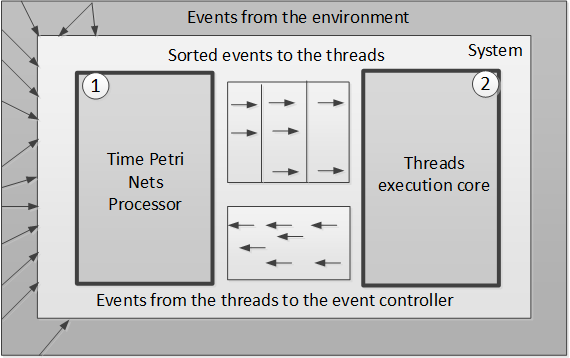
\includegraphics[width=0.85\linewidth]{./img/reactive_system}
			\caption{Reactive systems}
			\label{fig:reactive_systems}
		\end{figure}
		
		Module 1 from the Figure \ref{fig:reactive_systems} receive unsorted events from the environment
		and from the system itself. After the sorting of the events the Time Petri Nets processor
		transmits the result to the threads execution cores (module 2) of the system and the propers
		actions are taken\cite{peterson}. 
		
		In our system the fulfillment of program conditions is associated to sensitized transitions, 
		the resolution of a shot represents the fulfillment of those restrictions and if we associate 
		the request for verification of the conditions to a shot request, the resolution of a shot 
		communicates that conditions have been met.
		
		Definition: conditions for firing a transition from Time Petri Process:
		\begin{enumerate}
			\item The transition must comply with sensitization conditions named in Section
				\ref{subsec:sensitization_transitions}.
			\item The shot must be explicitly communicated by the processes or implicitly 
					recorded in the automatic shots module.
			\item Since it is possible that multiple transitions simultaneously satisfy the conditions
				described in paragraphs 1 and 2, the Time Petri Nets processor will execute first the
				firing with higher priority.\\
		\end{enumerate}	

		Figure \ref{fig:conection_multicore_system} show us how the Time Petri Nets processor is conected
		in a multicore system.
	
		In case that the firing of the transition can not be resolve, it is queued in the input queue, as
		shown in Figure \ref{fig:conection_multicore_system}, until the conditions of the system allow
		its resolution. The solution of the firing is notified to threads through the system bus, using
		the output queue. The threads of the system will execute the proper actions as indicated by 
		the firings that have been resolved, since the resolution of the firings depends on the Time 
		Petri Nets Processor state, which itself represents the state of the system.
	
		\begin{figure}[h]
			\centering
			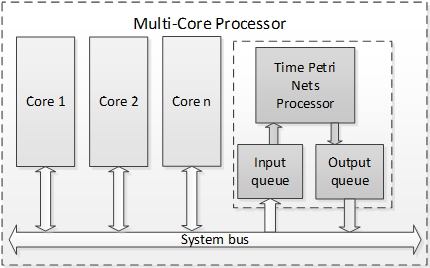
\includegraphics[width=.95\linewidth]{./img/conection_multicore_system}
			\caption{Multicore system with Time Petri Nets processor}
			\label{fig:conection_multicore_system}
		\end{figure}		




	%	Architecture
		\section{Time Petri Nets Processor Architecture and Operation}
	The processor executes the state equation solving only one firing of a transition at a time, this
	way it can solve all cases of firings, the simple ones (single firings) and the multiple firings, 
	performing as a single-firing sequence, as a result, the hardware is simpler.
	
	The resolution of firings is requested by the threads running on the cores through the system bus, 
	as emerging requests that system is running. These firing requests are received by the Time Petri 
	processor and stored in the input queue. This queue is FIFO according to each transition, the output 
	of this queue is a binary word which size equals the number of transitions. This word has ones in 
	the positions corresponding to transitions with firings requested. The order of the bit in the word 
	equals the number of transition over which the firing is requested. The bits that correspond to the 
	transitions which have no firing request are zero.
		
	\begin{figure}[h]
        \centering
        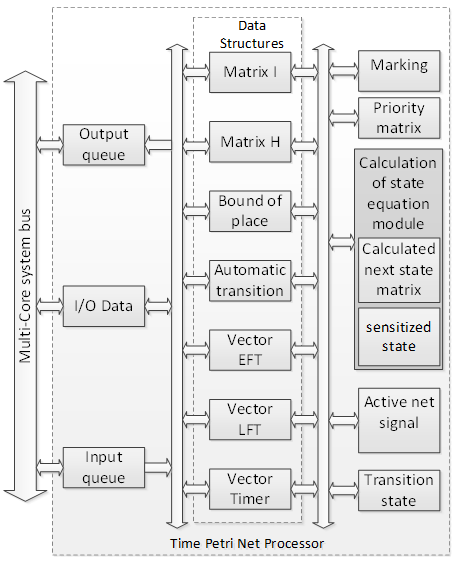
\includegraphics[width=0.95\linewidth]{./img/time_petri_nets_processor}
        \caption{Time Petri Nets Processor}
        \label{fig:time_petri_nets_processor}
    \end{figure}
    
    The output queue has a similar structure, but its function is to communicate to the threads those 
	firings that have been resolved.
	
	The data I/O module manages the access of the cores to the matrixes and vectors that program the 
	system. The module manages the access of the cores to the matrixes and vectors that program the system. 
	
	The matrixes and vectors described in the equation of state are the system program. This allows 
	us to program the processor directly from the Time Petri Net.
	
    Here we have added the inhibitor arcs matrix and the vector indicating the maximum number of tokens 
    in the places. This terms are not present in the state equations shown in this work but you can 
    consult the work\cite{paperProcesador}.\\
    
    The module in charge of solving the state equation of the Petri has the following responsibilities:
	\begin{enumerate}
  		\item Calculating the new state that would result from each transition firing only once, thereby 
  		generating a number of vectors calculated states equal to the number of transitions. Then, 
  		these vectors are stored. This is performed by subtracting the current state parallel to each 
  		column of $I^-$ and storing all resulting vectors, which will be evaluated to determine if 
  		the new state that each transition would produce is valid. This operation is performed whenever 
  		you change the time Petri Nets Processor status (current marking vector).
  		\item Determine which transition is sensitized. To do this, take all vectors calculated in 
  		step 1 and verify that there is no place to have a negative marking and neither exceeding the 
  		limit  of tokens it \footnotemark can hold.
  		\footnotetext{It is noted that this is a weak bound, since the marks in the squares are incremented 
	in step 4 and the limit is checked in step 2. This simplification facilitates hardware implementation.}
  		\item It starts or stops the timer. If a transition t has been sensitized and $Timer_t=0$ 
  		starts $Timer_t$, if $Timer_t\neq0$ does nothing.
  		\item Firing of one transition. Transitions that meet:
  		\begin{equation*}
			Vector EFT \leq Vector Timer_t \leq Vector LFT
		\end{equation*}				
		The transitions that meet that condition and have received one firing from input queue or 
		the firing programmed as automatic (which form a set of available firings).
		
		From that set, the firing with highest priority is selected and the transition is executed.
		
		According the executed transition, the state vector is actualized and the $Timer_t$  is 
		resetted to zero.
		\item Execute the steps 1, 2, 3 and 4 as a continuous cycle.\\
	\end{enumerate}	
	
	
	
	The system also has a unit that detects when no transition is sensitized and none $Timer_t$ 
	is higher than $LFT_t$. When this happens, the system generates an interruption notifying that 
	the system has finished its execution or is deadlocked. This feature is very useful to verify 
	the operation of the design and implementation of the system.
	
    
	% PERFORMANCE ANALYSIS
		\section{Performance Analysis}
	
	System implementation has been performed on a Atlys \texttrademark Spartan-6 Digilent platform \cite{atlys}, 
	cores used are the MicroBlaze v8.40 \cite{xilinx_microblaze} running an XilKernel v5.01a \cite{xilinx_xilkernel}
	operating system. Interconnected with Time Petri Processor by AXI bus\cite{xilinx_axi}.
	
	To verify the correct operation and analyze the IP Core synchronization times, measurements were 
	made for different numbers of iterations and number of threads trying to access a shared variable 
	in mutual exclusion. Then we compared the Petri Processor with an implementation using semaphores, 
	both solving the same problem. The choice of this second synchronization method is based on that 
	they are the lightest mechanism to perform these tasks.
	
	From these measurements, Speedup was calculated. The results are shown in Figure \ref{fig:speedup}, 
	where can be observed that for all cases, the processor is on average between 15\% and 30\% faster 
	than use of semaphores to solve the trouble of synchronizing multiple threads that want to accesses 
	a shared resource and even show peaks up to 70\%.
	
	These measurements were performed with times $\tau$ zero, in this way the performance is the same that i
	s obtained in the Petri Net Processor without temporal semantics. This is valid because the transition's
	time is part of the model, so, it is the same for the processor as for semaphore implementation.

		\begin{figure}[h]
			\centering
			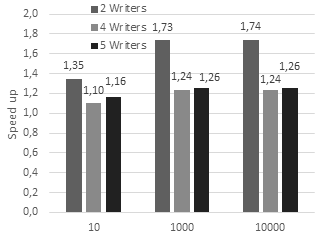
\includegraphics[width=0.85\linewidth]{./img/petri_speedup}
			\caption{Synchronization Speedup per iteration}
			\label{fig:speedup}
		\end{figure}
		
	As observed in Figure \ref{fig:simulation}, the processor needs only one half-clock cycle since the 
	counter reaches the value $\tau$ until a shot is placed in the output queue. The delay introduced is 
	insignificant in relation to the time takes a $\delta t$ of one clock cycle.
	
		\begin{figure}[h]
			\centering
			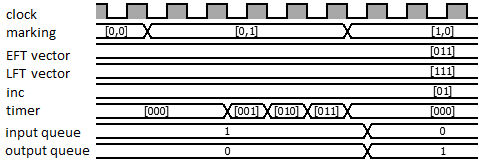
\includegraphics[width=0.95\linewidth]{./img/time}
			\caption{Running on hardware}
			\label{fig:simulation}
		\end{figure} 	
	
	Taking into account how insignificant the latency is and taking the time as part of the model it 
	is possible to analyze the performance without taking into account the vector $\Gamma$.	
	
	% IP Core Growth
		%%%%%%%%%%%%%%%%%%%%%%%%%%%%%%%%%%%%%%%%%%%%%%%%%%%%%%%%%%%%%%%%%%%%%%%%%%%%%%%%%%%%%
%																					%
%	TRABAJO: Paper Redes de Petri Temporizadas										%
%																					%
%		Titulo: 	Ejecucion de Redes de Petri Temporizadas						%
%																					%
%		Autores:	Julian Nonino													%
%					Carlos Renzo Pisetta											%
%					Orlando Micolini												%
%																					%
%	Seccion: IP core																%	
%	Archivo: ip_core.tex															%
%																					%
%%%%%%%%%%%%%%%%%%%%%%%%%%%%%%%%%%%%%%%%%%%%%%%%%%%%%%%%%%%%%%%%%%%%%%%%%%%%%%%%%%%%%
%	REVISIONES																		%
%																					%
%		19/10/2012																	%
%			Julian Nonino															%
%				Creacion de este archivo											%
%																					%
%%%%%%%%%%%%%%%%%%%%%%%%%%%%%%%%%%%%%%%%%%%%%%%%%%%%%%%%%%%%%%%%%%%%%%%%%%%%%%%%%%%%%
\section{IP cores}

		La arquitectura de este IP core se mantiene en su mayor parte igual a la de las versiones anteriores. 
		Con respecto a la versi�n que procesa \emph{Redes de Petri con Tiempo}, se quitaron los vectores \emph{EFT} 
		y \emph{LFT}, en su lugar se agreg� el \textbf{\emph{vector duraci�n}}. Se mantuvo el \textbf{\emph{vector de 
		incrementos de tiempo}} y el \textbf{\emph{vector de tiempo de sensibilizaci�n}}.
		 
		\subsection{Estructuras de datos para Redes de Petri Temporizadas}
	
		Como se muestra en la figura \ref{fig:diseno48} las estructuras de datos necesarias para la resoluci�n 
		de Redes de Petri Temporizadas son tres:
		\begin{itemize}
		  	\item Vector \textbf{\emph{duraci�n}}.
		  	\item Vector de \textbf{\emph{marcas temporales}}.
		  	\item Vector de \textbf{\emph{escala de incrementos de tiempo}}.
		\end{itemize}
		
		\begin{figure*}[!b]
			\centering
			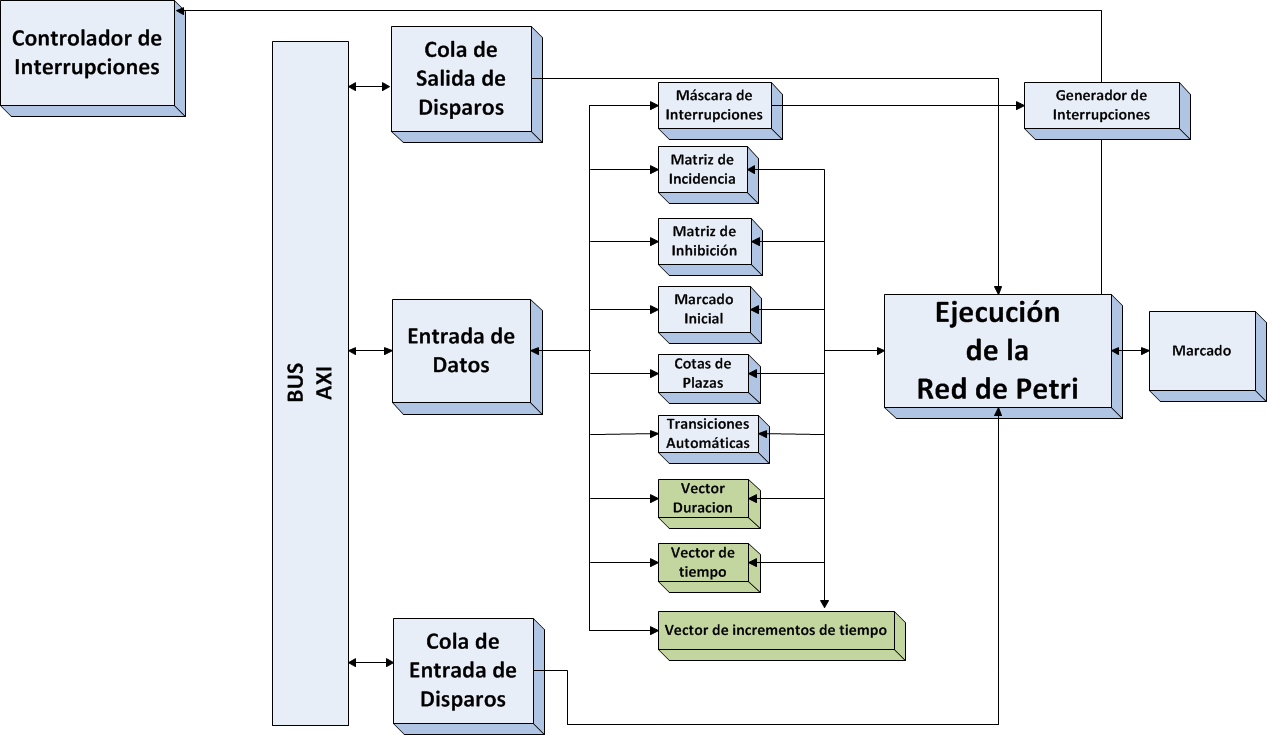
\includegraphics[width=6.5in]{./img/diseno48}
			\caption{Arquitectura del procesador de Redes de Petri Temporizadas}
			\label{fig:diseno48}
		\end{figure*}
		
		Los cuatro vectores tienen como cantidad de elementos el n�mero de transiciones. Los dos primeros son 
		tiene un tama�o de elementos parametrizable pero por defecto tienen 32 bits. El vector de escala de 
		incrementos de tiempo, por defecto toma el un tama�o de elementos de 5 bits.

		\subsection{Algoritmo de Ejecuci�n con Redes de Petri Temporizada}
	Basados en la teoria descripta se creo un algoritmo de ejecuci�n de disparos en una red de petri que se describe a continuaci�n es sintetizable en hardware y requiere 
	�nicamente 2 ciclos de reloj para ejecutar todos los pasos y a la vez permita un dise�o parametrizable en cuanto al tama�o y cantidad de elementos que soporte.

	\begin{enumerate}
		\item Espera de disparo en Cola de entrada de disparos.
		\item Llegado el disparo se calcula un vector binario de longitud cantidad de transiciones con un �nico 1 en el lugar correspondiente al n�mero de disparo, en funci�n del n�mero de transici�n que contenga. Este vector se utiliza para incrementar los contadores de disparos.
			Son considerados disparos en espera.
		\item Se calcula todos los posibles resultados para todos los disparos, hayan sido pedidos o no para confeccionar una matriz resultado donde cada columna Ci representa el nuevo marcado si la transici�n Ti  se disparara.
		\item Se crea una matriz de signos auxiliar con los signos correspondientes a cada elemento de la matriz resultado. 
		\item Se crea una matriz de inhibici�n auxiliar en funci�n del marcado actual y la Matriz de Inhibici�n determinando las plazas con arcos inhibidores que tienen tokens.
		\item Se crea una matriz de cotas en funci�n de la matriz resultados y las cotas de las plazas determinando cual fue superada para cada plaza por cada posible resultado
		\item Se crea un vector en el cual cada elemento corresponde a una columna de la matriz de signos y determina si esa transici�n es o no posible en funci�n si alg�n elemento de su resultado es negativo.
		\item Se crea un vector en el cual cada elemento corresponde a una columna de la matriz de inhibici�n y determina las transiciones que no pueden ser disparada debido a arcos inhibidores.
		\item Se crea un vector en el cual cada elemento corresponde a una columna de la matriz de cotas el cual determina que transiciones no pueden ser disparadas debido a que provocar�an superar las cotas de las plazas.
		\item En funci�n de los vectores creados en los puntos 7, 8 y 9 se crea un vector que determina las transiciones sensibilizadas. 
		\item Para determinar las transiciones a disparar se unen los disparos pendientes y las transiciones autom�ticas. Luego en funci�n de los disparos posibles y que la cola de disparos de salida no est� llena se actualiza el marcado �nicamente retirando tokens de las plazas  de entrada en funci�n de la matriz I-.
		\item Se habilita contador de transici�n temporizada.
		\item En cada clock de reloj se actualiza el vector de tiempo (contador saturado) de cada transici�n sensibilizada increment�ndolo seg�n el vector de incremento de tiempo correspondiente a partir de que la transici�n es disparada.
		\item Cuando el vector de tiempo supera la duraci�n de la transici�n se completa el disparo actualizando el marcado �nicamente agregando los tokens en las plazas de salida en funci�n de la matriz I+.
		\item Se incrementa contador de cola de salida correspondiente a transici�n ejecutada.
	\end{enumerate}		
	%	CONCLUSION
		\section{Conclusion and Contributions}

	In this paper, a Time Petri Processor is developed, which decouples the concurrency from sequential 
	processing, it has the following particularities:
	\begin{itemize}
  		\item On tasks, where measurements have been done, the processor allows synchronization of 
  				threads, with improvements up to 70\%.
		\item There is a direct relationship between the graph and the processor program, since this 
				is programmed with the state equation's matrixes and vectors.
		\item Multiple are admitted shots simultaneously in the same transition.
		\item Allows programming priorities since the shots are solved in parallel and are selected 
				according to priorities module.
		\item Decides if the shot can be executed or not in 2 clock cycles.
		\item The system programming is easier to do, since the processes are decoupled from the concurrency.
		\item This processor can be programmed at run time, thus it is possible to decrease the size 
				of the matrix in hardware by using spatial and temporal locality.
	\end{itemize}
	
	The difficulty of this implementation is because of the growth of the resources needed by the 
	increase of places and transitions. This implies that is difficult to implement a system for 
	dimensions greater than 32x32 in ZedBoard, to mitigate this difficulty new designs have been 
	proposed and are being worked on, these are: Petri Net Processor with pipeline architecture and 
	support for Hierarchical Petri Nets.

	% Conference papers do not normally have an appendix

	%	ACKNOWLEDGMENT
	%	% use section* for acknowledgement
\section*{Acknowledgment}

	The authors would like to thank...

	%	REFERENCES
		% Can use something like this to put references on a page
		% by themselves when using endfloat and the captionsoff option.
			\ifCLASSOPTIONcaptionsoff
		  		\newpage
			\fi
		% trigger a \newpage just before the given reference
		% number - used to balance the columns on the last page
		% adjust value as needed - may need to be readjusted if
		% the document is modified later
		%\IEEEtriggeratref{8}
		% The "triggered" command can be changed if desired:
		%\IEEEtriggercmd{\enlargethispage{-5in}}
		
		% references section
		
		% can use a bibliography generated by BibTeX as a .bbl file
		% BibTeX documentation can be easily obtained at:
		% http://www.ctan.org/tex-archive/biblio/bibtex/contrib/doc/
		% The IEEEtran BibTeX style support page is at:
		% http://www.michaelshell.org/tex/ieeetran/bibtex/
			\bibliographystyle{IEEEtran}
		% argument is your BibTeX string definitions and bibliography database(s)
			\bibliography{./bib/referencias}
		%
		% <OR> manually copy in the resultant .bbl file
		% set second argument of \begin to the number of references
		% (used to reserve space for the reference number labels box)
		%\begin{thebibliography}{1}
		
		%\bibitem{IEEEhowto:kopka}
		%H.~Kopka and P.~W. Daly, \emph{A Guide to \LaTeX}, 3rd~ed.\hskip 1em plus
		%  0.5em minus 0.4em\relax Harlow, England: Addison-Wesley, 1999.
		
		%\end{thebibliography}

	\end{document}
